
\section{Signs convention for fluid elements}

A fluid laminate with a lower $y$-coordinate exerts force on a fluid laminate with a bigger $y$-coordinate. With Newton's 3rd law we can therefore state that a fluid laminate with a bigger $y$-coorinate exerts negative force on a fluid laminate with a lower $y$-coordinate.

Similarly in the $x$-direction, a fluid element with a lower $x$-coordinate exerts force on a fluid element with a bigger $x$-coordinate and taking Newton's 3rd law, a fluid element with a bigger $x$-coordinate exerts negative force on a fluid element with a lower $x$-coordinate

\section{Newtonian fluids}



\section{Poiseuille flow}

Consider a steady-state flow of fluid between two parallel plates. We would like to find out what is the velocity and shear stress distribution along the $y$-axis.The pressure drop is assumed to be constant throughout the channel. This means that the pressure is a function of position $p = p(x)$ but the change in pressure per every equal distance in the channel is constant: $dp/dx = \text{const}$.

\begin{figure}[H]
\centering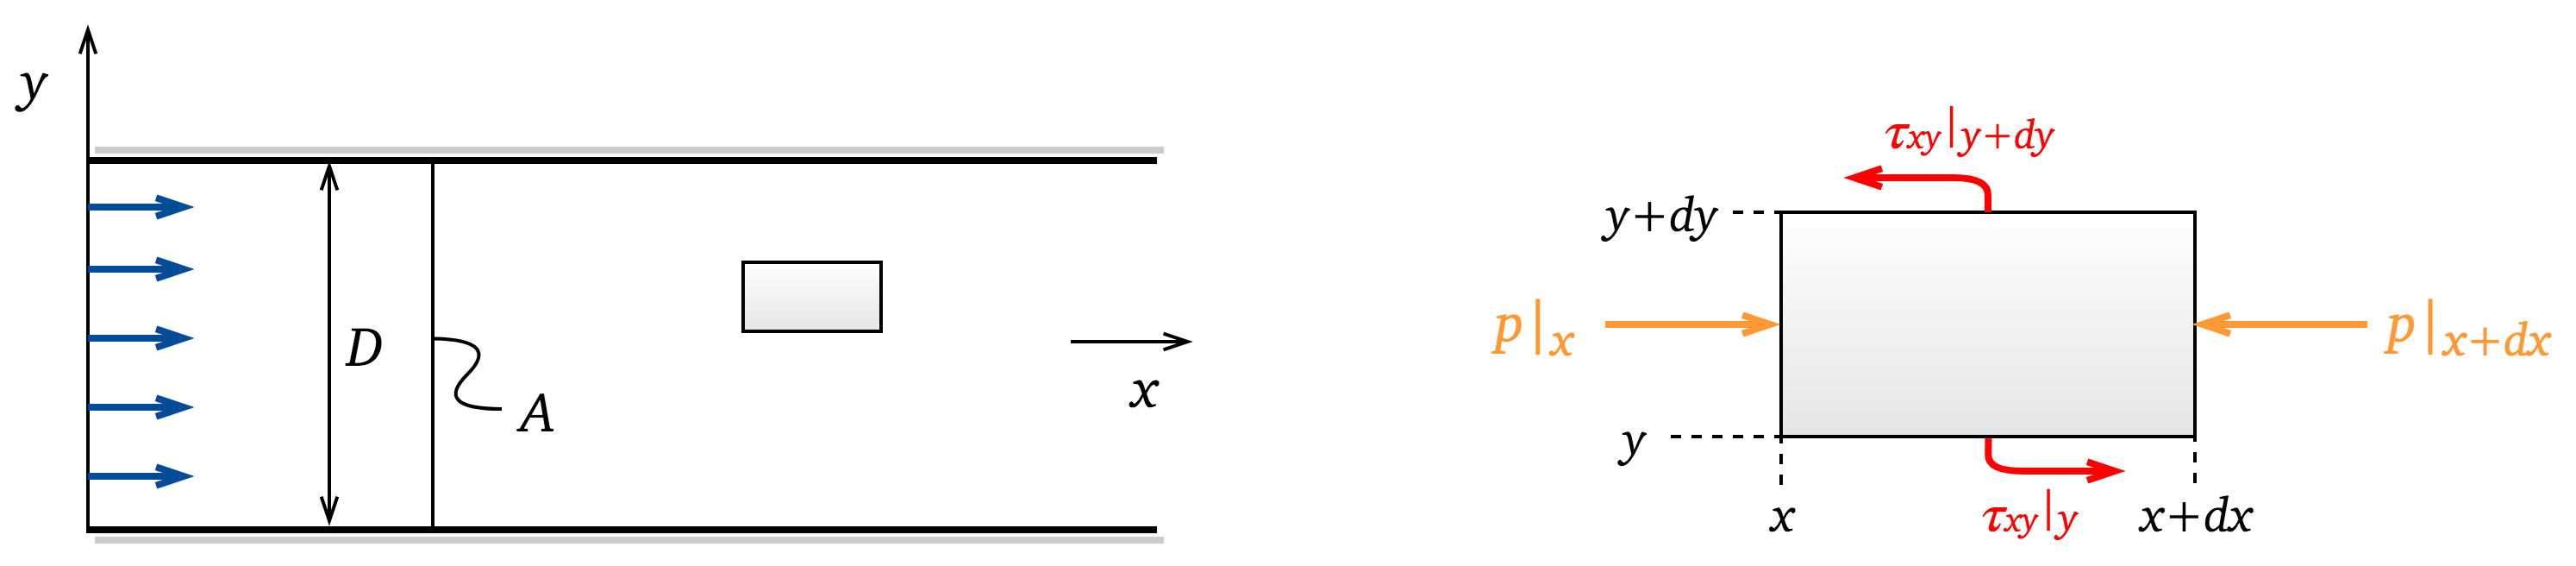
\includegraphics[width=14cm]{poiseuille-fluid-element}
\caption{Flow between two parallel plates with an infinitesimal fluid element.}			
\label{fig:poiseuille-fluid-element}
\end{figure}

We also have three boundary conditions. Due to a no-slip condition we assume that the velocity at the surfaces of the plates is zero: $\upsilon(-D/2) = 0$ and $\upsilon(D/2) = 0$. Due to symmetry of the situation, we assume that there cannot be any momentum transfer between the upper half and the lower half of the channel. Hence, the shear stress exactly in the middle of the channel is zero: $\tau_{xy}(0) = 0$.

Steady state momentum (force) balance, taking into account pressure and shear forces on a single infinitesimal fluid element:

\begin{equation}
0 = p|_x A dy - p|_{x+dx} A dy + \tau_{xy}|_y A dx - \tau_{yx}|_{y+dy} A dx
\end{equation}

Dividing both sides by the area $A$ and by $dx dy$ we obtain:

\begin{equation}
0 = \frac{p|_x  - p|_{x+dx}}{dx}  + \frac{\tau_{xy}|_y  - \tau_{yx}|_{y+dy}}{dy} 
\end{equation}

Now we notice that $\frac{p|_x  - p|_{x+dx}}{dx}$ is in fact equal to $\frac{dp}{dx}$, since it is an incremental change in pressure function value per incremental distance $dx$. Similar can be said about $\frac{\tau_{xy}|_y  - \tau_{yx}|_{y+dy}}{dy}$ which is equal to $\frac{d \tau_{xy}}{dy}$. We can thus further simplify:

\begin{equation}
0 = \frac{dp}{dx}  + \frac{d \tau_{xy}}{dy}
\end{equation}

\begin{equation}
\frac{d \tau_{xy}}{dy} = - \frac{dp}{dx} = \text{const}
\end{equation}

Integrating the above equation from $y = -D/2$ to $y = D/2$:

\begin{equation}
\tau_{xy}(y)= - \frac{dp}{dx} y + C_1
\end{equation}



